% sub-subsetion for 4.2.3 ----- ESTRATEGIA DE BUSQUEDA POR SNOWBALL
\subsubsection{Estrategia de Búsqueda 2: Bola de Nieve (Snowballing)}

\newcommand{\csiSelected}{24} %Estudios identficados con el SCI
\newcommand{\newSnowballStudies}{3} %Estudios obtenidos luego de aplicar criterios de inclusión y exclusión diseñados especificamente para el snowball.
\newcommand{\firstBackwardSnowballStudies}{3} %Primera iteración hacia atrás
\newcommand{\firstForwardSnowballStudies}{4} % Primera iteración hacia adelante
\newcommand{\secondBackwardSnowballStudies}{3} %Segunda iteracion haia atrás
\newcommand{\secondForwardSnowballStudies}{5} %Segunda iteración hacia adelante

%Total primer iteración.
\newcommand{\firstSnowballIterationStudies}{\fpeval{\firstBackwardSnowballStudies+\firstForwardSnowballStudies}}
%Total segunda iteración.
\newcommand{\secondSnowballIterationStudies}{\fpeval{\secondBackwardSnowballStudies+\secondForwardSnowballStudies}}

\newcommand{\snowballNewStudies}{\fpeval{\firstSnowballIterationStudies+\secondSnowballIterationStudies}}

La estrategia de búsqueda de bola de nieve comienza con la identificación del conjunto base de documentos a utilizar, seguido de una revisión y selección de documentos. La revisión consiste en verificar la lista de referencias mediante la identificación de nuevos documentos (bola de nieve hacia atrás). De manera similar, se identifican los documentos que citan el documento revisado (bola de nieve hacia adelante), lo cual requiere el uso de una base de datos que indique esta información. En todos los casos, la sección de documentos aplica los criterios de exclusión \cite{Wohlin-01}.
Esta estrategia comprende dos pasos. El primer paso se denomina ``Construcción de línea base de bola de nieve'' y se enfoca en establecer estudios para iniciar el análisis de referencias y citas. Para la composición de este conjunto de estudios, utilizamos varios criterios basados en el CVI (Índice de Valor de Contenido), SCI (Índice de Citas de Estudios), además de también usar la inclusión directa. El segundo paso se denomina ``Selección de estudios'', y se enfoca en el análisis de referencias (Bola de nieve hacia atrás) y citas (Bola de nieve hacia adelante) de cada estudio.


% Snowball baseline building 
\bolditalic{Construcción de línea base de bola de nieve}: Basándonos en los \screenTot{} estudios seleccionados durante la fase de screening, se realizó un análisis exhaustivo de frecuencia y relevancia académica mediante el cual se evaluó la calidad e impacto científico de cada publicación. A través de la aplicación sistemática del índice SCI  como criterio de selección por calidad, se logró identificar y extraer \csiSelected{} estudios de alta relevancia que constituyen la base fundamental para la implementación de la estrategia de búsqueda por bola de nieve. Estos estudios seleccionados, caracterizados por su alto índice de citación y reconocimiento en la comunidad científica, servirán como punto de partida para las iteraciones de snowball hacia adelante (\textit{forward snowballing}, es decir, aquellos trabajos citados en nuestros estudios base) y hacia atrás (\textit{backward snowballing}, esto es, aquellos trabajos que citaron nuestros estudios base), permitiendo así expandir la búsqueda bibliográfica de manera dirigida hacia literatura de calidad comprobada en el dominio de los universos HTCondor.

\bolditalic{Selección de estudios}: Para esta actividad se decidió hacer dos iteraciones de bola de nieve. Se comienza con la primera iteración hacia atrás revisando en cada uno de los \csiSelected{} estudios semilla. Esta revisión permitió identificar nuevos artículos que cumplen con nuevos requisitos de inclusión fabricados para este proceso. Ver Figura \ref{figure:Snowball}. Así pues, la primera iteración se hizo el proceso de bola de nieve hacia atrás, lo que permitió obtener \firstBackwardSnowballStudies.  Posteriormente se realiza la iteración hacia adelante, revisando aquellos estudios que citan los documentos de línea base, obteniendo como resultado \firstForwardSnowballStudies{}.

\begin{figure}[htbp]
	\centering
	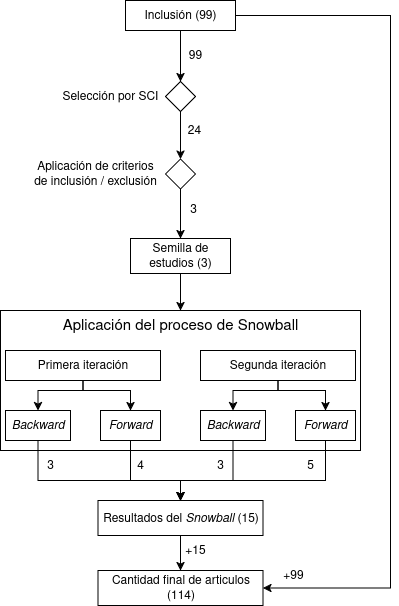
\includegraphics[scale=0.55]{resources/figures/sms-Snowball.drawio.png}
	\caption{Estrategia de búsqueda por bola de nieve.}
	\label{figure:Snowball}
\end{figure}

Para la segunda iteración se obtuvieron \secondBackwardSnowballStudies{} para la bola de nieve hacia atrás y \secondForwardSnowballStudies{} para la bola de nieve hacia adelante, consiguiendo así otros \secondSnowballIterationStudies{}.


Esta actividad se realizó a través de Google Scholar y siguiendo la práctica en el estudio \cite{Ali-01}. El resultado conseguido fueron \snowballNewStudies{} nuevos estudios.

% -------- Tabla : Criterios de inclusión/exclusión ------------
\begin{table}[htbp]
	\centering
	\caption{Criterios de inclusión/exclusión}
	\label{table:inclusion_exclusion_criteria}
	\renewcommand{\arraystretch}{1}  % Increase row height globally
	\begin{tabular}{p{1.5cm}p{2.2cm}p{3.9cm}}
		\toprule
		\textbf{Categoría}           & \textbf{Inclusión}         & \textbf{Exclusión}                                                                                                          \\
		\midrule
		\textbf{Tipo de publicación} & Artículos de investigación & Tesis, capítulos de libros, libros, revistas, conferencias, y todo lo demás que no esté en el tipo de publicación inclusiva \\
		\addlinespace[0.8em]
		\textbf{Período}             & Desde 2020 hasta 2024      & -                                                                                                                           \\
		\addlinespace[0.8em]
		\textbf{Idioma}              & Inglés                     & -                                                                                                                           \\
		\bottomrule
	\end{tabular}
\end{table}
% --------------------------------------------------------------
